\documentclass[a4paper,10pt]{article}
\usepackage[margin=2.5cm, nohead]{geometry}
\usepackage{graphicx}
\usepackage{hyperref}
\usepackage{verbatim}
\usepackage{color} % for todo
\usepackage{subfig}
%\usepackage{fancyhdr}

% TODO, make this pretty!
%\setlength{\parskip}{10pt}
%\newcommand{\todo}[1]{\colorbox{red}{\color{white}#1}}
%%\setlength{\headheight}{15.2pt}
%\pagestyle{fancy}
%%\rfoot{\footnotesize{\name + \title}
%%\lfoot{\footnotesize{\name}}
%\cfoot{\footnotesize{Awesomizing the P2DX: AP2DX}}
%%\lhead{\course}
%%\rhead{\title}
%\pagestyle{fancy}
%\renewcommand{\headrulewidth}{0.2pt}
%\renewcommand{\footrulewidth}{0.2pt}

\title{Reflection Report AP2DX}
\author{Maarten Inja}


\newcommand{\todo}[1]{\colorbox{red}{\color{white}#1}}

\begin{document}
\maketitle

\section{Forming team AP2DX}
For the project ``Software Engineering \& Gedistribueerde Applicaties'' a team was formed of five people. 
While the project is part of second year of the bachelor computer science at the UvA, no students in the 
team actually studied computer science. Three study Artificial Intelligence, one studies 
Computer Science and ICT at the Amsterdam University of Applied Sciences and one studies for the 
pre-master Software Engineering. Even though none of the team members were in the target group for this
project, morale was high and initial expectations were even higher.

The goal of the project was to write software for a simulated \emph{P2DX} robot. This software would
allow the robot drive autonomously. So, naturally, we named our team ``Awesomizing P2DX''. Or, shorter
: ``AP2DX''. It was
figured that this was what the team was going to do. 

The group members at the start of the project:
\begin{itemize}
    \item Waddie Assal, 6398693 (studies Computer Science and ICT) 
    \item Maarten Inja, 5872464 (studies AI)
    \item Jasper Timmer, 5995140 (studies pre-master Software Engineering)
    \item Jeroen Rooijmans, 5887410 (studies AI)
    \item Maarten de Waard, 5894883 (studies AI)
\end{itemize}

\section{Week 1}
The first weeks secretary was Waddie Assal. Tasks for this week included; creating a work plan, planning
and familiarizing ourselves with the software we had to deal with the coming month. For example the USAR simulator, 
a version control system. 

The team also decided to lunch together each day. Two different team members would bicycle to
the local Albert Heijn each day to buy delicious lunch goods. This way, team enjoyed excellent lunch
each day of the project for the rest of the project. Having lunch together was also considered to be great for the team spirit and good
for team building.

Group meetings went well and connecting to the simulator was surprisingly easy. We designed a framework and the
baseclass on a whiteboard (see figure \ref{fig:whiteboard}) which was something we hold on to till the very end
of our project. We even started programming and had a build server running.

\begin{figure}[h]
\centering
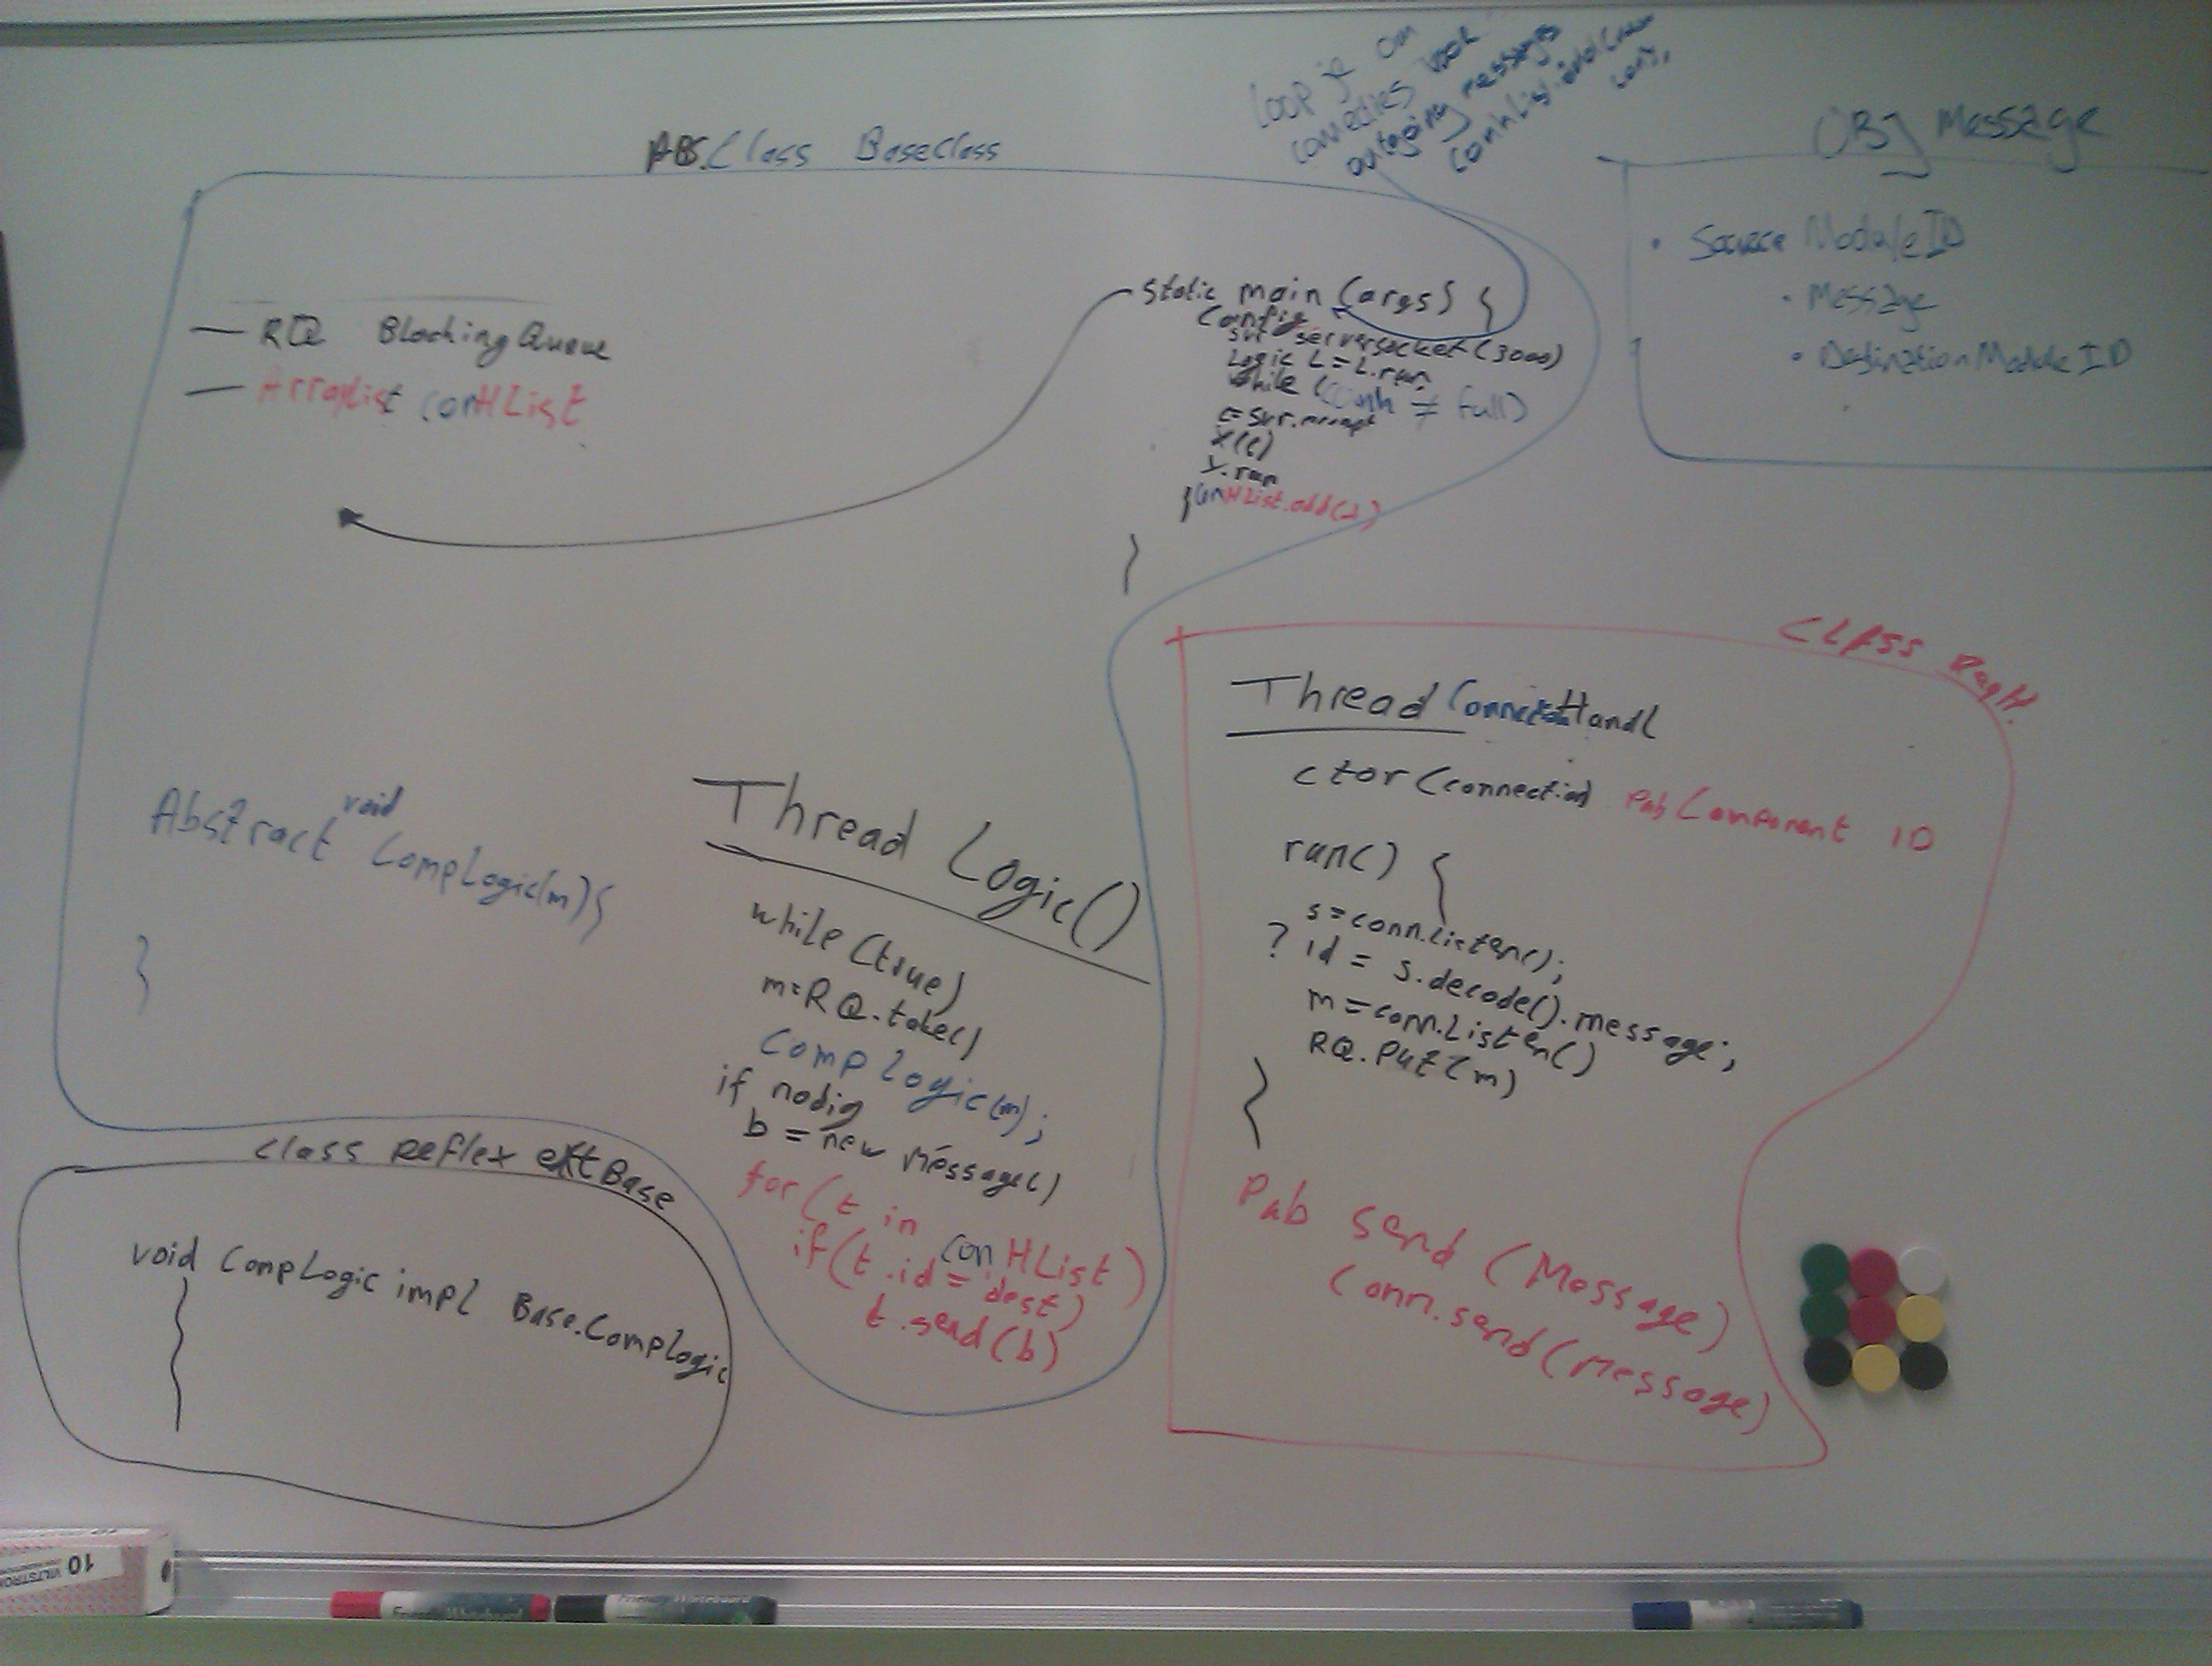
\includegraphics[width=12cm]{whiteboard}
\caption{It might look sloppy but it actually wasn't}
\label{fig:whiteboard}
\end{figure}

However, not everything was sunshine and happiness, Jeroen Rooijmans got sick at Thursday and went on a sail 
weekend on Friday. This left us with four people halfway through the first week already! It 
was agreed that he would improve the work plan on Monday the next week. 

\section{Week 2}
The second weeks secretary was Jeroen Rooijmans. Monday was pentecost and the university was closed. 
Tuesday work was resumed. Jeroen Rooijmans wrote one page for the final version of the work plan in two days time 
(Monday and Tuesday) and went absent and later sick the rest of the week. The other team members resumed
programming, wrote tests and implemented things such as the base class and message protocols. Especially writing tests 
classes was hard.
We were new at this and it soaked up a lot of time. Eventually we figured it out and
it started to work, but with one
team member short and the deliverable being in the now near future programming was given a (much) higher
priority. 

On Friday, the day of the deadline of the first deliverable, we had nothing to show for our hard work. We wrote
an e-mail to Jeroen Rooijmans explaining how we felt that he did not show enough commitment. We had decided to 
have him write all the tests for our project. Individually he could have no excuses and his work could be measured
in percentages (and even seen in graphs). He also had taken up the task of writing the report for the first deliverable. 

\section{Week 3}
The third weeks secretary was Jasper Timmer. 
It turned out Jeroen Rooijmans had failed to write a good report. At least, we thought so. He had mixed up English 
and Dutch in the same file and basically bluffed that we had reached the goals of the deliverable. We were not amused. 

The first two days of week three both Wadie Assal and Jeroen Rooijmans were sick and absent. The three team members left
were a bit frightened of failing the project. We had not really accomplished anything, the debugging of the framework
went really slowly and we only had three people left! 

Luckily Wadie Assal was back at Wednesday (taking over the task of writing the tests for now) and Jeroen Rooijmans quit our team. 
We were able to meet the goals of the first deliverable at the date of 
the second deliverable. 

\section{Week 4}
The fourth weeks secretary was Maarten de Waard. With the framework running we rushed to implement a mapper and 
the robot movement. Things went really fast and goals were met in short amounts of time. Only Maarten Inja 
went home sick for half a day, on Wednesday afternoon. (Which was a new record for our team, just half a day in a week).
The other team members prepared for the presentation and demonstration and finished work on programming the robots
movement behavior and mapping ability.

On Thursday we presented and demonstrated our work. 

On Friday we wrote the report. 

\end{document}



















